\chapter{Roman Jakobson and the theory of distinctive features}
\label{ch.jakobson}

During his years in Czechoslovakia, and especially in the thirties,
{\Jakobson}'s views on phonology were developed very much within the
context of his cooperation with {\Trubetzkoy} and the other members of
the Prague school. If {\Jakobson} was clearly the leading spirit of this
partnership in many ways, it is still somewhat difficult to
disentangle his individual contributions from {\Trubetzkoy}'s in those
years; and as with the relation between {\Kruszewski} and {\DeCourtenay} during their `Kazan period', it is probably unprofitable to
attempt to do so. Of course, the two disagreed on many points (mostly
of detail), as attested in their letters; but it was only after
{\Trubetzkoy}'s death in 1938 that {\Jakobson}'s own position began to
diverge in significant ways from that underlying their earlier
collaborative work.

\begin{wrapfigure}[10]{r}{.35\textwidth}
  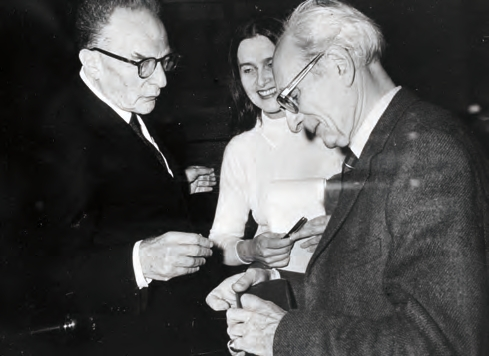
\includegraphics[width=.9\textwidth]{figures/jakobson.levi-strauss.jpg}
  \caption{Roman Jakobson and Claude Levi-Strauss (1972)}
  \label{fig:ch.jakobson_jakobson_levi-strauss}
\end{wrapfigure}
In March 1939, shortly after the {German} invasion of Czechoslovakia,
{\Jakobson} managed to escape to Denmark.\footnote{For a more detailed
  account of {\Jakobson}'s travels to escape the Germans, see
  \citealt{efj97:jakobson}.} After only a few months it became clear
that this was no real refuge, and he went to Norway; when Norway was
occupied in its turn, he went to Sweden, where he stayed until
1941. In that year he managed a perilous journey by sea to New
York. During 1942-46 he was active in what had become the {French}
University in exile, the École Libre des Hautes Études. He was in
close contact there with other European émigrés, including the
anthropologist \name{Claude}{Levi-Strauss}, who was greatly taken with the
possibilities of applying `structuralist' methods derived from
linguistics (as he learned it from {\Jakobson}) to the social sciences
more generally.

{\Jakobson} was welcomed by important American linguists, including Franz
{\Boas}, \name{Leonard}{Bloomfield} and \name{Zellig}{Harris}, all of whom tried to help
him find an appropriate academic position, though without success
\citep{swiggers91-93:jakobson}.  He was by no means universally
acclaimed in the United States, however. On the one hand, he found
some of his old anti-structuralist opponents from Europe who had
similarly taken refuge there. Partly by the sheer force of his
personality, he was quite able to dominate these less positive
influences; and he and a new generation of his students quickly became
central to the discussions of the {Linguistic Circle of New York}
(founded in 1943 on the model of the Prague Linguistic Circle) and to
much of the work published in its new (1945) journal \textsl{Word}.

On the other hand, he also encountered opposition from other Americans
\citep{dixon07:jakobson.2dollar.bills}. Some of this seems to have
been based purely on regrettable and not always very subtle
xenophobia, but much also represented a genuine conflict of scientific
views. By comparison with the radical positivist and operationalist
climate of thought among the members of the `post-Bloomfieldian'
generation (which we will treat below in
chapter~\ref{ch.structuralists}), then dominant in the Linguistic
Society of America and in American universities, {\Jakobson}'s position
seemed wildly idealistic. By insisting on the importance of
unobservable `meanings' (the \emph{\isi{signifié}} of the linguistic sign)
as well as the supposedly `hard data' of acoustic phonetic fact (the
\emph{\isi{signifiant}}), {\Jakobson} seemed to threaten a retreat into what
many American linguists considered more of a recidivist metaphysics of
language than proper `science'.

Even the most patently `scientific' (because highly technological)
aspect of {\Jakobson}'s position—the appeal to data from acoustic
research, which had progressed greatly by the end of the 1940s—was
widely considered illicit. This was because of the use he made of it:
in proposing a universal system of phonological description founded on
properties that could be defined independent of particular languages,
{\Jakobson} threatened the position of presupposition-less, fundamentally
agnostic analysis that many believed was essential to objective
\isi{linguistic description}.

Although they did not succeed in changing the basic directions of
American linguistics overnight, {\Jakobson} and his students continued to
gain prominence and influence, representing in some ways the `official
opposition'. American linguists' hostility toward Europeans abated
somewhat in the early 1950s: \citet{hockett51:review.martinet}
published a favorable review of {\Martinet}'s work, and {\Hjelmslev} taught
in the 1952 {Linguistic Institute}. {\Jakobson} was elected president of
the {Linguistic Society of America} for 1956, representing in some ways
the seeds of a fundamental reorientation of research away from an
increasingly sterile obsession with purely procedural
issues. Especially among Slavists, though, {\Jakobson} had already become
a genuinely central figure by that time.

In 1946, he had been appointed to the Thomas G. Masaryk Professorship
of Czechoslovak Studies at Columbia. In 1949 he was appointed
professor of Slavic and general linguistics at Harvard, and in 1957
(on the strength of his interest and work in the acoustic structure of
speech) he also became professor (later Institute Professor) at
MIT. He continued to be associated with both institutions (though
forced to retire officially from Harvard in 1967 at the mandatory
retirement age of seventy) until his death in 1982.

\section{Origins of the distinctive feature theory}

Most of the central aspects of {\Jakobson}'s view of phonological
structure can be identified in the prewar Prague school picture
presented in {\Trubetzkoy}'s \textsl{Grund\-züge}, a work which {\Jakobson}
had seen through to pulbication after {\Trubetzkoy}'s death, but their
elaboration nonetheless resulted in a distinctly individual
position. This position was taken over in largely intact form by (at
least early work in) generative phonology, and it is important to be
clear on its basic elements and their motivation.

{\Trubetzkoy}'s theory was, as described in chapter~\ref{ch.prague},
primarily a theory of systems of phonemes: ideal segment-like
constructs reduced to their distinctive minimum, and identified only
by their opposition to the other elements of the same system. Although
he says in places that phonemes should be regarded as composed of
features (which would seem to imply logically that features, not
pho\-nemes, are the minimal building blocks of \isi{sound structure}), this
formulation is due to {\Jakobson} and in some ways foreign to the actual
thrust of {\Trubetzkoy}'s work. He seems to have regarded the individual
features that are the basis of phonemic \isi{oppositions} more as
characterizations of the dimensions along which systems of phonemes
are structured than as actual units having autonomous ontological
status.

This is perhaps a rather subtle distinction: if the phonemic units of
{\Trubetzkoy}'s analyses are identifiable only in terms of the
distinctive dimensions along which they are opposed to other units,
the difference between this and saying that the properties themselves
are the basic units, combined into clusters of simultaneously
co-occurring elements which are in turn concatenated sequentially,
seems more a matter of philosophical than of linguistic
significance. Nonetheless, {\Jakobson}'s insistence that it is features,
not phonemes, that are the fundamental units of linguistic analysis
represents a conceptual break with {\Trubetzkoy}'s position. In a paper
presented to a group of linguists in Copenhagen (but only published
much later), \citet{jakobson39:struktur} stressed the fundamental
nature of the distinctive properties of phonemes, as opposed to the
larger units composed of them. This change of perspective has
significant consequences for the range of issues addressed by the
theory.

\begin{wrapfigure}{l}{.35\textwidth}
  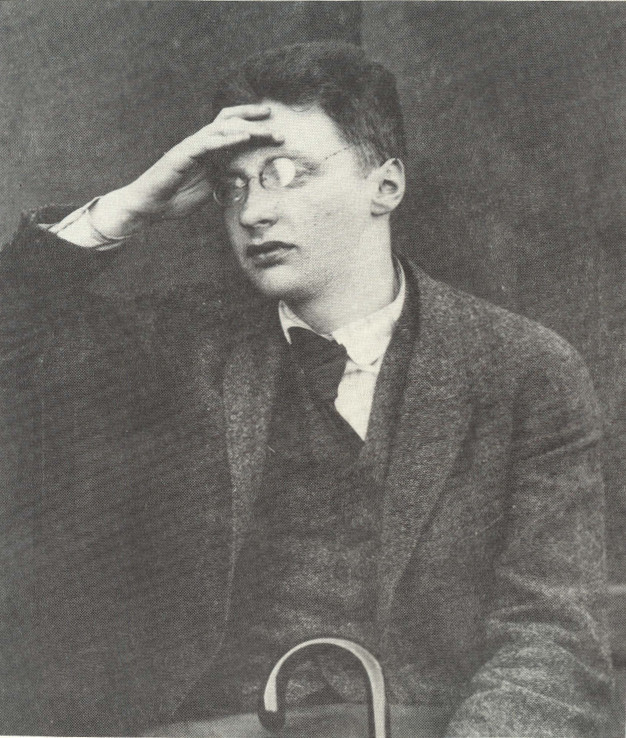
\includegraphics[width=.9\textwidth]{figures/RomanJakobson-1920.jpg}
  \caption{Roman Jakobson in 1920}
  \label{fig:ch.jakobson_jakobson_1920}
\end{wrapfigure}
In {\Jakobson}'s view, {\Saussure} was fundamentally mistaken in a number of
his basic propositions about the nature of language. We have already
had occasion (in section~\ref{sec:backgr-prag-circle}) to note
{\Jakobson}'s opinion that it was misleading for {\Saussure} to {stress} the
absolute separation of synchronic and diachronic aspects of language,
since this would rule out a teleological interpretation of change in
terms of the properties of the system undergoing it. In
\citet{jakobson29:remarks}, he discusses a wide range of
sound changes in the early history of Slavic that can only be
understood collectively in terms of the overall properties of the
linguistic systems within which they arise and to which they lead.  He
also took exception, however, to what {\Saussure} regarded as two of the
most basic properties of the linguistic sign.

One of these was the claim that linguistic signs have an essentially
sequential character, which {\Jakobson} took to imply an analysis that
{stops} with units the size of the segment. According to his own
position, it is necessary to continue the analysis until the
autonomous simultaneous components are reached. This is in essence
only a matter of degree of precision, comparable to the decomposition
of morphological elements into phonemes after words have been analyzed
into morphemes, rather than a fundamentally different procedure; but
nonetheless not one that can be allowed to be impeded by an insistence
on a purely linear arrangement of the constituents of the sign.

Second, {\Jakobson} felt that the doctrine of the \isi{arbitrariness} of the
sign had to be subjected to important qualifications. While it is of
course true that signs are arbitrary in that the link between a
particular \emph{\isi{signifié}} and a particular \emph{\isi{signifiant}} is
established by the conventions of the \isi{linguistic system}, this does not
imply that the sorts of things that can serve as potential \isi{signifiants}
are constrained only by the necessity to be different from one
another. In particular, language has an essentially spoken character,
as a result of which the \emph{\isi{signifiants}} are necessarily to be
found in their logically primary form in the structuring of
sound. Furthermore, not just any differences in sound are potentially
relevant phonologically: a universal inventory can be given of the
small set of \isi{distinctive features} that function to differentiate
\emph{\isi{signifiants}} in natural languages. Insofar as the
\emph{\isi{signifiant}} of any sign in any language must be made up of these
same elements, the \isi{arbitrariness} of the sign is considerably
restricted.

Of course, if this view is to have cogency, it is necessary to
establish a plausible set of candidates for the status of universal
\isi{distinctive features}. These features must be defined generally enough
to be applicable to the wide range of phonetic phenomena observed to
differentiate forms in the languages of the world; but precisely
enough to make specific claims about what is and is not a possible
\isi{phonological system}, thus giving the theory empirical content. Much of
{\Jakobson}'s writing on phonological topics was directed precisely
toward refining the proposed inventory of these universal features.

The system of {\Trubetzkoy}'s \textsl{Grundzüge} can fairly be described
as the first attempt to provide such a universal framework of the
features that are exploited for phonological purposes in the languages
of the world (as opposed to purely phonetic descriptive
frameworks). The set of parameters proposed there involved a fairly
large number of features. Each was provided with a general,
language-independent definition, but some of these definitions were
articulatory in character while others were based in \isi{acoustics}. Within
the overall framework of segmental features, different sets were
proposed for vowels and for \isi{consonants}. The proposed classification of
\isi{oppositions} allowed for a number of different types, including for
instance both bilateral and multilateral \isi{oppositions}.

In all of these respects, {\Jakobson}'s views gradually came to
differ. {\Jakobson} reports that he and {\Trubetzkoy} had already differed
by 1938 on the issue of whether truly multilateral \isi{oppositions} should
be recognized. Seeking a framework which would provide a maximally
uniform notion of phonological opposition, he noted that most of the
features in the \textsl{Grundzüge} system were in fact bilateral, and
suggested that those few that apparently were not might actually be
decomposable into two or more bilateral \isi{oppositions} (a proposal of
which {\Trubetzkoy} appears to have remained unconvinced). In 1938
{\Jakobson} developed his position in a talk to the Prague Linguistic
Circle, and subsequently at the International Congress of Phonetic
Sciences in Ghent.

In this paper, \citet{jakobson39:classement} considers the most
obvious candidate for a multilateral opposition, the parameter of
\isi{place of articulation} in \isi{consonants}. All previous descriptive
frameworks had treated the differences among labial, dental, palatal,
and velar \isi{consonants} (as well as those at other positions) as
completely parallel, aligned along a single dimension. {\Jakobson}
proposed, however, that this apparent uniformity in fact represented
(at least) two distinct features.

One of these, differentiating labials and velars on the one hand from
dentals and palatals on the other, can be defined both in articulatory
and acoustic terms. \emph{Grave} \isi{consonants} (labials and velars) are
formed with a relatively large, undivided oral resonant cavity,
resulting in a relatively low frequency region of prominence in their
acoustic spectrum; while \emph{acute} \isi{consonants} (dentals and
palatals) are formed with an oral cavity divided into two smaller
resonators, resulting in a relatively high-frequency region of
spectral prominence.

Cross-classifying with this difference is that between
\emph{posterior} (later called \emph{compact}, in keeping with a
preference for acoustic over articulatory terminology) \isi{consonants}
(velars and palatals), formed with a constriction relatively far back
in the mouth, and \emph{anterior} (later called \emph{diffuse} for the
same reason) \isi{consonants}, the labials and the dentals which are formed
with a relatively front constriction. In acoustic terms,
\citet{jakobson39:classement} identifies compact \isi{consonants} only by
their relatively greater perceptibility; in subsequent formulations,
they were described as having a concentration of energy in the central
region of the acoustic spectrum (as opposed to diffuse \isi{consonants},
which lack such a concentration). Regardless of their specific
definitions, however, if these features are accepted, the result is a
theory in which the multilateral opposition of place is replaced by a
pair of binary \isi{oppositions}, supporting the possibility that
multilateral \isi{oppositions} can perhaps be dispensed with entirely.

\section{Developing the theory of distinctive features}

At least three major points follow from this analysis: the logical
character of the \isi{distinctive features}, the substantive nature of their
definitions, and the homogeneity of their application to sounds of all
classes. Each of these represents an important theme in {\Jakobson}'s
later work.

First, of course, is the exclusive role played by binary \isi{oppositions}
in the resulting theory. {\Jakobson} consistently argued that the
principle of binary \isi{oppositions} is absolutely fundamental to language,
and has its basis in the nature of our mental processes. He notes
later that individual nerve cells appear to function on a strict
`on/off' basis, and suggests that this property is reflected in the
structure of language (though he does not discuss the fact that the
muscles which actually implement articulatory gestures are by no means
binary in their control possibilities).

With the reduction of consonantal \isi{place of articulation} to a set of
binary \isi{oppositions}, this program is largely accomplished in the domain
of phonological features. Additional \isi{place of articulation}
distinctions beyond the basic four (e.g., the difference between
velars and uvulars) are argued to be treated in terms of other binary
properties. He claims, for example, that \isi{uvular} \isi{stops} in most
languages are actually \isi{affricates}, and thus relatively
\emph{strident}—noisy, or affricated—by comparison with velars. There
is thus no need to recognize a distinct uvular point of \isi{articulation}
for \isi{consonants}, since an independent dimension is available to
\isi{contrast} \isi{uvular}s with other sounds.

One further candidate for the status of a multilateral opposition must
also be mentioned, in part because its status continues to be
controversial. The difference among high, mid, and low vowels (perhaps
with still further height distinctions) is much less easily decomposed
into binary features than is consonantal point of \isi{articulation}. One
proposed solution was to make use of additional properties (similar to
the use of stridency mentioned above for \isi{consonants}): many height
distinctions, for example (such as [i] vs. [ɪ]), can evidently be
reduced to differences in \emph{tenseness}. There still appear to be
at least three irreducible degrees of vowel quality distinguished only
by height, however. To describe these, {\Jakobson} at one point proposed
that a single feature was involved, but that it took three values: + ,
$-$, and ± (or perhaps 0, for `unspecified'). Yet this is
transparently not a binary opposition in any interesting sense, and
most presentations of {\Jakobson}'s framework rely on dividing the
parameter \emph{compact}/\emph{diffuse} into two features: [±compact]
and [±diffuse], with mid vowels specified as [$-$compact, $-$diffuse].

Another important aspect of the theory presented in
\citet{jakobson39:classement} and subsequent work is its striving to
provide every feature with definitions in both articulatory and
auditory terms. Relying on the fact that language is in its essence a
spoken system, {\Jakobson} surmised that its primitive terms must have an
objective, external basis in the acoustic signal as well as in the
articulatory activity of the speaker (and the auditory perception of
the hearer). In practice, the transformations from \isi{articulation} to
\isi{acoustics} and from \isi{acoustics} to \isi{articulation} are not unique (since
more than one articulatory configuration can give rise to the same
sound, and the same configuration can produce more than one sound);
therefore, what we really want, in addition to these, is an auditory
or perceptual definition, since we speak in order to be understood.

This insistence that the \isi{distinctive features} are identifiable
directly in the signal at all three stages (articulatory, acoustic,
and perceptual) limits the range of properties that can be encompassed
to those with a direct surface realization. Whatever their importance
in other terms (e.g., \isi{morphophonemics}), abstract differences between
forms cannot count as `phonological' in the strict sense. We will
explore in chapter~\ref{ch.structuralists} some of the motivations
behind this limitation of phonology to surface properties (which is of
course not at all limited to {\Jakobson}'s position); for {\Jakobson}, it
seems to follow directly from the basis of language in speech
communication, and the need to provide simultaneous objective
definitions of features at all \isi{levels} of the speech communication
process.

Another important aspect of {\Jakobson}'s position which is already
present in his first major paper on phonology after {\Trubetzkoy}'s death
is what we might call the `one mouth' principle: the requirement that
the same apparatus be used to describe both vowels and \isi{consonants}
simultaneously, rather than providing separate sets of features for
these two classes of sounds. The division between grave and acute
\isi{consonants} is first presented as parallel to that between grave and
acute vowels (the grave vowels being back, and the acute vowels
front); and the three \isi{consonants} {[p, t, k]} are said to be arranged
perceptually in a triangle which is quite parallel to the \isi{vowel}
triangle of {[u, i, a]}.

Such a parallel is obviously suggested by the insistence on an
acoustic and auditory perspective, and not only an articulatory
one. If this proposal is to be realized, however, it is necessary to
frame the definitions of the \isi{distinctive features} in rather general
terms, so as to make them applicable simultaneously to the rather
different structure of \isi{vowels} and \isi{consonants} (as well as the
intermediate classes of glides and liquids).

This elimination of the difference between features for \isi{vowels} and
features for \isi{consonants}, in its turn, paves the way for the most
striking aspect of the {\Jakobson}ian system. As a general program, this
system assimilates as many traditional phonetic dimensions as possible
to one another, bringing them together under a single general
definition wherever this is possible and they cannot be shown to
function independently of one another. The result is a radical
reduction of the number of features recognized (from around forty in
{\Trubetzkoy}'s system to roughly a dozen), and a much greater
utilization of this minimal set of dimensions in the languages of the
world—potentially leading to a richer universal theory of phonological
systems and their structure.

Some of the reduction in the number of \isi{distinctive features} in
{\Jakobson}'s system is provided by framing definitions in terms of
relative, rather than absolute properties. The import of this is that
each feature is defined in terms of a general, language-independent
set of properties—but the segments distinguished by a given feature
may still be determinable only on a language-particular basis.

For example, \citet{jakobson62:retrospect} cites the fact that
\ili{Bulgarian} has two vowels in each of the following classes: front
unround (/i/. /e/, back round (/u/, /o/), and back unround (/ə/,
/a/). The three classes can easily be distinguished by means of the
features grave/acute (separating back from front vowels) and
flat/nonflat (separating rounded from unrounded vowels). Within these
classes, however, the question of the appropriate way to characterize
the distinctions involved remains, /i/ and /u/ are high vowels, /e/,
/ə/, and /o/ are mid, and /a/ is low; so we would appear to have to do
with three vowel heights. But {\Jakobson} argues that in each class we
really have to do with a difference between a relatively higher (more
diffuse) vowel and a relatively lower (more compact) vowel—and thus we
can differentiate the members of each pair by the same feature,
without regard to the fact that the [+diffuse] member of the [+grave,
$-$flat] pair (namely, /o/) is actually articulated at the same height
as the [$-$diffuse] members of the other two sets.

The fact that features are to be interpreted as distinguishing
segments in terms of their relative (rather than absolute) possession
of some property has important consequences for the general program of
making maximal use of a minimal set of potentially contrastive
dimensions. It can also be regarded as a way of encoding certain
information about rule-governed \isi{variation} into the definition of
elements of a phonological representation, similar to the role played
in {\Trubetzkoy}'s theory by the \isi{archiphoneme} and the \isi{morphoneme} (see
chapter~\ref{ch.prague}). As should be evident, {\Jakobson}'s theory is
just as much a theory of \isi{representations} as {\Trubetzkoy}'s, with little
explicit place for a notion of `rule' except in the definition of
elements of these \isi{representations}.

The role of relative feature definitions in this program is clear from
{\Jakobson}'s examples. For instance, he often cites the fact that in
\ili{Danish}, initial [t] and [d] \isi{contrast}, while post-vocalically we find
[d] and [ð]. By interpreting the opposition in both positions as one
between a relatively tense and a relatively lax obstruent, we obtain
the desired result of identifying initial [t] with post-vocalic [d],
and initial [d] with post-vocalic [ð]. But another way of looking at
the same analysis is to observe that, by treating features as defined
relatively, we are able to provide a uniform phonological
representation for certain sets of phonetically distinct segments [t]
and [d], [d] and [ð]) which alternate with one another under definable
conditions. The definitions of the phonemic elements /t/ and /d/ and
their opposition thus incorporate what is in effect a rule of
post-vocalic lenition. Such analyses are subject to the constraint that
the alternating segments be sufficiently similar to one another
phonetically for the device of relative feature definitions to be
sufficient to describe their relation; but this still allows a
considerable range of \isi{variation} that might be described by rules that
convert one segment type into another to be described directly in
terms of constant representational elements.

The program of collapsing phonetically distinct contrasts into a
single phonological dimension was already important in
\citet{jakobson39:classement}. In that paper, for instance, it was
suggested that a distinct \isi{place of articulation} did not have to be
provided for \isi{affricates} since these could be distinguished from plain
\isi{stops} in the same general articulatory/acoustic region by means of the
property of \emph{stridency} (noisy release). The same parameter also
can be used to make other place-of-\isi{articulation} distinctions such as
that between bilabials and labiodentals, between alveolars like
\ili{English} [s] and interdentals dike \ili{English} [θ], etc.; and as already
noted, since uvulars in most languages are more affricated than the
corresponding velars, this distinction too can be included under
stridency.

In {\Jakobson}'s later development of the distinctive feature system,
several other features subsume a number of phonetically distinct
dimensions. The most dramatic of these, perhaps, is the feature
[±flat] \citep{jakobson.fant.halle52:preliminaries}, which includes
distinctions of (a) rounding, (b) \isi{retroflexion}, (c) velarization, and
(d) pharyngealization. The feature [±checked], in its turn,
encompasses ejection, implosion, and clicks.

In each case, an important empirical claim is made by bringing the
several contrasts under a single feature, to the effect that no
language will ever display two or more of the contrasts covered by a
single feature independently. Of course, this does not mean that a
language cannot, for example, have both rounded and retroflex
\isi{consonants} (since both would \isi{contrast} with plain \isi{consonants} by being
[+flat])—but only that the two cannot be independently contrastive
under otherwise identical conditions. Thus, the \isi{contrast} of
\isi{retroflexion} might appear in dental \isi{stops} and \isi{fricatives}, and rounding
in velars, without violating the claim made by the definition of the
feature [Flat].

\section{The adequacy of Jakobson's distinctive features}

The limited inventory of very general features which form the system
presented in {\Jakobson}'s work
\citep{jakobson.fant.halle52:preliminaries,cherry.halle.jakobson53:logical,jakobson.halle56:fundamentals}
can be seen to make very strong empirical claims about the range of
possible phonological systems in natural languages. When these claims
are taken seriously in the investigation of a wide range of languages,
the results pose a number of problems for the Jakobsonian system.

For example, a number of languages in Australia have \isi{stops} and nasals
at six points of \isi{articulation} \citep{butcher.fletcher14:australian}:
labial, interdental, alveolar, post-alveolar (retroflex), palatal, and
velar. The labial, palatal, and velar positions pose no problems, but
apparently all of the interdental, alveolar, and post-alveolar segments
must be treated as [acute, diffuse]. The feature [flat] can be used to
distinguish the post-alveolar position from the others, but the
interdental and alveolar positions remain unseparated. While the
feature [strident] might be called into play for this purpose in the
case of the \isi{stops}, this is obviously unsuitable as a description of
the difference between interdental and alveolar nasals, and the
Jakobsonian system does not seem to provide any more adequate
alternative.

A variety of languages present logically similar problems. \ili{Chipewyan}
\citep{cook04:chipewyan}, for example, is reported to \isi{contrast} two
\isi{affricates} in the dental/alveolar region [t͡s] vs. [t͡θ]); since
stridency is already employed to separate \isi{affricates} from the
corresponding \isi{stops}, it is not available to make this further
distinction as well. Also, as with the problem posed by the Australian
systems noted above, some languages (e.g., dialects of West
Greenlandic, \citealt{rischel74:greenlandic}) present a \isi{contrast}
between velar and uvular nasals which cannot plausibly be described as
based on stridency. It appears, then, that more points of \isi{articulation}
must be recognized than the four basic ones provided by the
Jakobsonian system; and at minimum, this entails the addition of some
further features (assuming the framework of binary \isi{oppositions} is
maintained).

There are also some problems for the generalization represented by the
definition of the feature [flat]. The definition of this feature
predicts that no language will have more than one independent \isi{contrast}
out of a set consisting of rounding, \isi{retroflexion}, velarization, and
pharyngealization. In some northwest Caucasian languages
\citep{colarusso88:nwc_phonology} including \ili{Ubykh} and (the Bzyb
dialect of) \ili{Abkhaz}, however, independent contrasts of \isi{retroflexion} and
rounding are reported among \isi{affricates} in the alveopalatal
region. \ili{Ubykh} also displays independently contrastive plain, rounded,
pharyngealized, and rounded-pharyngealized uvular \isi{stops}. Bzyb \ili{Abkhaz}
has uvular \isi{fricatives} of five distinct types: plain, rounded,
`palatalized' (involving an increase in the length of the
constriction), pharyngealized, and rounded-pharyngealized.

A \isi{contrast} of rounding is also reported for distinctively pharyngeal
\isi{fricatives} in some languages of the Salishan family, such as Okanagan
\citep{pattison78:okanagan}.  In vowel systems, the Northeast
Caucasian language \ili{Tsakhur} \citep{schulze97:tsakhur} has a vowel
system including two high back vowels ([ɨ] and [u]) that \isi{contrast} in
rounding (as well as [i], [e], [a] and [o]); each of these vowels
appears with contrastive pharyngealization as well.

From the above observations, we can conclude that several of the
detailed claims made by the Jakobsonian feature system concerning the
complementarity of certain contrasts are not borne out. For most of
the cases in which two or more traditional phonetic dimensions are
united under a single feature in this system, in fact, it is possible
to find languages in which these dimensions are independently
contrastive. On the other hand, we should not let this cause us to
lose sight of the somewhat marginal nature of such cases: the
problematic contrasts are exhibited only in languages of rather
unusual structure, such as those of the Northwest Caucasus and the
Northwest coast of North America, languages which are noted for their
exuberant consonantal inventories. As generalizations about the vast
majority of the world's languages, the complementarities predicted by
the Jakobsonian system are overwhelmingly valid, although they fail as
claims about the range of possible systems in natural languages.

A different sort of objection to the comprehensive adequacy of the
Jakobsonian system for the description of natural languages is due
originally to \citet{mccawley67:features}. He points out that a
complete description of any language within such a system would
require not only a set of \isi{phonological representations} for forms, but
also a set of principles (a) supplying the values of redundant
features; and (b) interpreting the \isi{distinctive features} in terms of
their particular articulatory and acoustic realization. That is, given
the fact that a given segment is characterized as e.g. [+flat], it is
still necessary to specify whether this means that it is rounded,
pharyngealized, retroflexed, or velarized. This set of principles
specifying the non-distinctive aspects of speech may be impossible to
formulate in a satisfactory way if it is based on \isi{representations}
given in a system like {\Jakobson}'s.

To illustrate this problem, {\McCawley} cites facts from \ili{Arabic}. \ili{Arabic}
has a set of pharyngealized \isi{consonants} (the `emphatics') which are
contrastively [+flat]; it also has three vowels /a/, /i/, and /u/
which involve a rounding \isi{contrast} and thus another use of the feature
[flat]. The contrasts involved are not independent (rounding is only
contrastive in vowels, and pharyngealization only in certain
\isi{consonants}), so a problem of the sort discussed in the preceding
paragraphs does not arise; but another difficulty appears as a result
of certain non-distinctive facts about \ili{Arabic} pronunciation.

In particular, vowels adjacent to a pharyngealized consonant are
predictably pharyngealized themselves. To describe this, we might say
that vowels become (predictably) [+flat] when preceded or followed by
a [+flat] consonant. But when we now come to interpret the feature
[+flat], we need to say the following: (a) in \isi{consonants}, [+flat]
means `pharyngealized'; (b) in vowels that are high and back,
[+flat] entails `rounded'; and (c) in vowels adjacent to
pharyngealized \isi{consonants}, [+flat] entails `pharyngealized'. The
problem, of course, is that this last statement duplicates the
principle by which [flat] is redundantly assigned to vowels adjacent
to [flat] \isi{consonants}. Other formulations of the specific rules
involved could be proposed, but there does not appear to be any
description which does not involve such a duplication.

This argument bears on the adequacy of the Jakobsonian feature system
so long as we accept the assumption that the same set of features
(including [flat]) is to be employed both to specify the contrastive
values of the \isi{phonological representations} of forms and the
nondistinctive or redundant properties of their pronunciation. In
numerous places {\Jakobson} insists that a description of the redundant
features as well as the distinctive ones must be included in an
adequate theory of language; and he never proposed a real theory of
these redundant features which would be separate from the theory of
\isi{distinctive features}. The assumption might thus be warranted that he
intended to employ the same set of features to describe both
distinctive and redundant properties.

As {\McCawley} points out, this is exactly the assumption adopted by
{\Halle} in such early generative work as \citet{halle:spr}, and indeed
quite generally until the revisions in the basis of the feature system
proposed in \citet{spe}. Nonetheless, {\McCawley}'s argument from \ili{Arabic}
makes it clear that whatever the value of the Jakobsonian framework
for the description of the distinctive properties of phonemic forms,
an adequate treatment of the relation between these forms and actual
pronunciation must be based on a somewhat different set of features
which do not involve collapsing distinct but complementary phonetic
properties under a single dimension of \isi{contrast}.

Once we see that such a (non-minimal) set of general phonetic
parameters plays an essential role in the description of natural
language systems, we must then ask what the motivation is for assuming
a separate, minimal set of specifically \isi{distinctive features}. For
{\Jakobson}, such a special status for the system of \isi{distinctive features}
is motivated by the unique status of the \isi{representations} which they
characterize: \isi{representations} in which only the distinctive properties
of a form are registered, with all predictable or redundant
information rigorously eliminated.

Of course, if it were true that no language could employ, for example,
both rounding and \isi{retroflexion} independently, then characterizing any
particular \isi{contrast} as phonologically one or the other would leave
this \isi{predictability} unexpressed; and so the conflation of
complementary features forms an integral part of the definition of
phonemic forms as strictly distinctive, and non-redundant. In
{\Jakobson}'s view, the existence of a level of representation defined by
exactly this property of non-\isi{redundancy} follows directly from the
Saussurean insight that the linguistic significance of a form lies in
the way it differs from other forms. Non-redundant phonemic
\isi{representations} characterize these differences directly and
explicitly, thus apparently expressing the linguistic essence of
particular forms.

The absence of predictable features from the essential nature of the
linguistic \isi{signifiant} appeared self-evident to {\Jakobson}. Directly
echoing {\Trubetzkoy}'s rejection of {\Baudouin}'s conception of the \isi{phoneme}
as the psychological equivalent of a \isi{speech sound},
\citet{jakobson.halle56:fundamentals} argue that such a psychological
picture is based on a fallacy: ``we have no right to presume that the
sound correlate in our internal speech or in our speech intention is
confined to the \isi{distinctive features} to the exclusion of the
configurative or redundant features.''

The extension of this observation to the claim that utterances should
be provided with a distinct phonemic form devoid of all configurative
or redundant features rests on the assumption that phonological theory
is fundamentally a theory of \isi{representations}, and that the only way to
characterize limitations on the \isi{variation} that does or does not count
as corresponding to the `same' linguistic unit is by defining a level
of representation that will have exactly that property. If, as we have
argued above (in chapter~\ref{ch.saussure_sound}), it is also possible
to characterize this \isi{variation} and its limits by means of rules that
relate \isi{representations} not specifically defined by this property, then
the motivation for a separate system of distinctive (as opposed to
more generally phonetic) features disappears along with the necessity
of such a level of representation.

We might still motivate the Jakobsonian system of a minimal set of
phonetic features by the argument that, even though this specific
proposal about their substantive content may be in need of refinement
and revision (as the observations above about their empirical adequacy
suggest), it is still overwhelmingly the case that many phonetic
dimensions are in overall \isi{complementary distribution} in natural
languages. Thus, even though a tiny minority of languages do indeed
exploit both rounding and pharyngealization separately, most treat
only one or the other (or, obviously, neither) of these as potentially
contrastive under any given set of circumstances. If a fully adequate
set of features along Jakobsonian lines could be constructed, this
might allow us to express such generalizations about natural language.

Before admitting a set of features constructed on this basis, however,
we must ask exactly what the insight is that characterizes it. In
fact, the possibility for generalization in the Jakobsonian system
rests essentially on the auditory foundation of the features
themselves. This suggests that what is really at issue here is a
rather direct pragmatic fact, rooted (as {\Jakobson} so often insisted)
in the basis of language in speech communication. We could formulate
the relevant generalization approximately as follows: the more nearly
similar two phonetic parameters are in their auditory correlates, the
less likely they are to function as independent cues to the identity
of particular forms.

Put in such a way, the generalization appears to be almost a truism:
the harder it is to distinguish which of two properties is intended,
the harder it is to use them independently as cues to the intended
form of an utterance. By showing that, for example, all of the
properties brought together under the proposed feature [flat] are
highly similar in their acoustic consequences, {\Jakobson} and his
coworkers provided just this basis for the observation that these
properties are by and large not treated as independent cues in
perceptual identification, and thus in the structure of languages.

But, of course, this generalization is a relative one and not
absolute: as long as two properties are not absolutely identical in
their acoustic and auditory consequences, there is still the
possibility that they will show up in some language as
independent. This is exactly the case with the wide range of
auditorily marginal distinctions exceptionally exploited by languages
like those of the Northwest Caucasian family; and the fact that these
cues are usually reinforced in such languages by other (redundant)
ones simply stresses the unusual nature of the situation.

Indeed, the role played by this generalization is considerably broader
than that of simply predicting what contrasts can co-occur within a
given phonemic system. When we state it not in terms of (surface)
distinctive properties, as in {\Jakobson}'s system, but in terms of the
perceptual cues used to identify linguistic forms, it has other clear
consequences for the evolution of phonological systems.

For example, there is no serious question that the properties of
\isi{voicing} in obstruents and \isi{tone} in vowels constitute quite independent
dimensions of \isi{contrast}, which must be separated in any adequate
framework for phonological description even though both rely on
control of laryngeal \isi{articulation}. Nonetheless, both of these have the
property that one of the acoustic cues utilized in their perception is
the frequency (in relative value or direction of change) of vocal cord
vibration. As is well known, voiced obstruents induce a lower \isi{pitch} on
the immediately following portion of a vowel, and (certain kinds of)
voiceless obstruents induce a relatively higher \isi{pitch} in the same
way. Though attempts have been made to attribute both of these effects
to the same features, there are excellent reasons to assume that they
are quite independent \citep{sra78:tone_features,tang08:tone}.  It
happens, however, that the articulatory mechanisms involved in
controlling obstruent \isi{voicing} have as side effects a perturbation of
the frequency of vocal cord vibration. Further, there is some evidence
to the effect that such perturbations can be among the cues utilized
perceptually for the identification of obstruents as voiced or
voiceless. The role of fundamental frequency in the case of
distinctions of \isi{tone} is obvious.

Thus, we have to do with two independent dimensions of \isi{contrast}, which
happen to have some auditory similarity (in that they share in part a
perceptual cue) and articulatory interaction (in that they are
grounded in the same components of the speech production
apparatus). We must, of course, recognize a basic distinction between
the phonological properties in question and the auditory cues which
allow a listener to identify them: otherwise, we would be unable to
describe the independence typically shown by \isi{tone} and
\isi{voicing}. Equally, however, we must recognize the consequences of the
auditory relationship which such a shared cue establishes between
properties. To the extent that they are both identifiable (at least in
part) on the basis of evidence from the acoustic value F₀, the
independence of \isi{tone} and \isi{voicing} is likely to be compromised in the
same way as that of the various properties brought together by
{\Jakobson} into a single feature on the basis of a (nearly) uniform
auditory definition.

In this case, we can see the action of the generalization above in the
fact that, in the evolution of a number of languages (especially in
the Sino-\ili{Tibetan} family), \isi{voicing} distinctions have been reinterpreted
as distinctions of \isi{tone} (and perhaps vice versa, though this is more
controversial). The \isi{mechanism} involved is evidently the following:
given the auditory similarity between the two, they are likely to be
interpreted as related rather than independent; and at that point, a
property other than the originally intended one may be taken to be the
independent variable. The \isi{pitch} perturbations provoked by \isi{voicing}
distinctions were at some point reinterpreted as representing
autonomous tonal contrasts, and the change in phonological structure
is thus a consequence of the auditory relation between the two
parameters. We see here the effect of the same generalization that
accounts for those instances of complementarity between phonetic
dimensions which {\Jakobson}'s system attempts (in too absolute a
fashion) to capture. {\Jakobson}'s insight concerning the importance of
auditory considerations is a very real one, but it is relevant to
other areas than the delimitation of a universally adequate feature
system for phonological description.

\section{\textsl{Kindersprache, Aphasie und allgemeine Lautgesetze}}

Although the development of {\Jakobson}'s thought in regard to the system
of \isi{distinctive features} took place over a long period, its high point
was perhaps his \citeyear{jakobson:kindersprache} monograph on child
language, \isi{aphasia}, and phonological \isi{universals}. The work was written
in Norway, while he was more or less constantly on the move before
settling in the United States. It attempts to bring together facts
from a wide variety of areas whose relationship we now take for
granted (largely as a result of {\Jakobson}'s ideas) but which were then
treated by rather different disciplines. The purpose of this
enterprise, of course, was to bring this putatively extralinguistic
material to bear on the analysis of synchronic phonological systems,
to enable us to understand on a more general basis what is `natural'
about natural languages, or why they are as they are. This was
undoubtedly the first attempt within modern linguistics to create a
genuinely explanatory theory of linguistic systems by establishing
logical and empirical connections between the data of linguistic
analysis \emph{per se} and other, independent domains.

At the time {\Jakobson} wrote, the available data concerning language
acquisition, language dissolution in \isi{aphasia}, the general bases of
auditory perception, and other areas to which he refers were largely
fragmentary from a linguistic point of view. As a result, some of his
factual assertions about language cannot stand as empirically valid
today; but if the linguistic relevance of this material is now much
better understood, and the available data much greater both in
quantity and quality, it is primarily because of the wealth of
suggestive implications {\Jakobson} found in what was available to him in
1941. It is a considerable tribute to his insight that, if the ensuing
eighty years of research have revised many points of detail, the broad
outlines of his bold synthesis continue to be confirmed.

He begins with the study of the most obviously linguistic material
available (which was, however, largely the result of studies by
non-linguists): the course of acquisition of a first language by
children. It is necessary first of all to argue that this material is
indeed linguistic in character: that is, that the deviations in
children's early speech from the system of adult language really are
based on linguistic principles and have a systematic character which
is relevant to the understanding of linguistic systems, rather than
being based merely on physical, perceptual, or conceptual limitations
inherent in uncompleted development. While one cannot of course
completely neglect the influence of such limitations (where they can
be shown to exist), {\Jakobson} argues that the vast majority of
deviations in child speech that had been recorded could in fact be
understood and organized by the terms and categories of linguistic
systems; and that they thus represent authentically and systematically
different systems rather than simply imperfect command of the adult
system.

{\Jakobson} also notes that the data of language change support the
relevance of \isi{child language} to adult language. When we examine the
sorts of change found in the evolution of a variety of languages, we
often find that they correspond closely to the reductions or changes
shown by \isi{child language} with regard to its adult model. This suggests,
of course, that much of language change has its basis exactly in these
alterations made by the child: that the child's innovations are in
some instances taken up and continued in adult systems, and that this
forms an important source of raw material for change. The systematic,
linguistic nature of the modifications made by the child is shown by
the fact that, in many instances, it cannot be claimed that sound
types altered in early language are at all unpronounceable (and thus
due to possibly extra-linguistic limitations of development). They may
well appear elsewhere in the system as modifications of other sounds,
and in any case many modified sounds are well attested in earlier
stages of the child's development.

The proposal that change has its roots in \isi{child language} was not new
with {\Jakobson}: \citet{grammont02:child.language,grammont33:traite}
among others had earlier observed striking similarities between the
two, and devoted considerable attention to them as a source of data
for his theory of change. There are also some remarks by {\DeCourtenay}
that can be seen as recognizing the relevance of child
language for the class of anthropophonic processes which, as discussed
above in chapter~\ref{ch.kazan}, serve as the foundation of all
alternations in adult language systems. Nonetheless, {\Jakobson}'s use of
these connections is more ambitious than that of his predecessors. He
wants not simply to refer to observations about \isi{child language} as a
factual source for a theory of linguistic change: he wants rather to
establish the point that adult language systems are as they are
because they necessarily develop in a particular systematic way that
can be studied in the form of \isi{child language}.

{\Jakobson} notes that before the onset of genuine meaningful language,
the child goes through a stage of `\isi{babbling}', in which typically a
vast array of sound types are produced (including such comparative
exotica as clicks, \isi{nasal vowels}, obstruent liquids, etc.).  More or
less suddenly, however, this enormous diversity disappears, to be
replaced by a radically reduced inventory of sounds in the child's
first real words. This corresponds, according to {\Jakobson}, to the
transition from a stage in which the \isi{babbling} is pure sound, pure
expression, to a point at which sound production is employed in the
service of expressing a distinctive function. Babbling can be regarded
as serving the purpose of a sort of preliminary `tuning up' of the
articulatory and auditory apparatus, establishing the range of
gestures of which this apparatus is capable and their acoustic
consequences, but without utilizing the resulting sound for any
(non-emotive) meaningful expression. As soon as sound comes to
constitute the \emph{\isi{signifiant}} of a linguistic sign associated with
a \emph{\isi{signifié}}, however, a fundamental {change} takes place in the
range of productions thus utilized. Where once nearly any sound from
nearly any language could be found in the child's babblings, the first
words typically involve very few: [p], [m], and [a], in particular.

This radical reduction in variety had largely confounded earlier
attempts to ascribe a systematic course to language development: how
can it be that, if children are observed to produce \isi{nasal vowels} at
six months, such sounds appear to be beyond the capacity of a two-year
old? For {\Jakobson}, the answer is clear: after the \isi{babbling} period,
when language becomes endowed with distinctive function, it is not the
articulations of sound types that need to be developed, since these
are already well established. Rather, it is the use of distinctive
\isi{oppositions} that is lacking, and this must be built up piece by
piece.

Evidence for this proposition comes from several sources. First, of
course, the fact that post-\isi{babbling} language acquisition does not
consist in acquiring the articulatory skill to produce a wide variety
of sounds is shown by the very diversity of content of \isi{babbling}
itself. Second, however, even during the period of development of
genuine language, the child often gives evidence of controlling a
wider variety of articulations than are available for distinctive
exploitation. Frequently, sounds that are missing from the child's
meaningful language nonetheless appear in purely expressive uses
(interjections, onomatopoeia, imitations, etc.). Further, a sound that
is missing in one class of words may well appear in others as a
substitute for some other sound, when a sort of `chain shift' of
segments occurs.

The essential point {\Jakobson} draws from these data is that the process
of developing the system of distinctive uses of sound is qualitatively
quite independent of the development of mere articulatory
control. Furthermore, once the issue is clarified in this way and
attention focused on the emergence of a genuinely \isi{linguistic system} of
sound values, a striking conclusion emerges: the order of development
of sound distinctions is roughly constant across languages, in a
sequence independent of the nature of the language being acquired.

Thus, all children begin with a minimal opposition of a single vowel
(roughly [a]) and a single consonant (generally labial
[p]). Consonantal distinctions arise with a difference between a nasal
([m]) and an oral ([p]) segment type; and subsequently with a split in
point of \isi{articulation} between grave (labial) and acute (dental)
sounds. Within vowels, the first split is between compact (low) and
diffuse (high) segments. With regard to \isi{manner of articulation}, \isi{stops}
arise before \isi{fricatives}, and both before \isi{affricates}. The
consonant/vowel distinction precedes the emergence of liquids or
glides, and sonorant liquids precede obstruent liquids. Some
distinctions, where they are to appear, arise only very late: e.g.,
nasal vs. oral vowels; \isi{oppositions} between liquids; non-pulmonic
airstream mechanisms (ejectives, \isi{implosives}, clicks,
etc.).

The uniformity of the sequence in which these segmental distinctions
are acquired seems quite general.\footnote{Much more information about
  the sequence in which children develop their phonological systems
  has accumulated in the years since \citealt{jakobson:kindersprache}
  was written, of course.  Generalizations of the sort {\Jakobson} sought
  and their import for a variety of phonological theories have been an
  important area of research in the field
  \citep{rose.inkelas11:child.language}, a topic largely initiated by
  his ideas.} Of course, a child acquiring a language which does not
have a given opposition obviously does not introduce it simply because
it is the next thing in the chain of development. The predictive role
of these generalizations is relative to the set of \isi{oppositions} present
in the language ultimately to be acquired: their sequence follows
strict lines (though some of these lines, such as those governing
e.g. vowel quality and consonantal manner distinctions, may be largely
independent of one another) which (for any given set of \isi{oppositions})
are related in the same way in the development of any language.

An important corollary of the determinacy of this developmental
sequence is the prediction it makes about possible phonological
systems. Since the child must acquire \isi{stops} before \isi{fricatives}, and
both before \isi{affricates}, the prediction is made that a system with only
\isi{fricatives} and not \isi{stops}, or with \isi{stops} and \isi{affricates} but no
\isi{fricatives}, could not be acquired, since an essential step toward the
development of such a system would in each case be missing. Now in
fact there are languages with \isi{stops} but no \isi{fricatives} (many languages
in Australia, for example), but not vice versa; and while there are
many languages with \isi{stops} and \isi{fricatives} but no \isi{affricates}, there are
no languages attested in which \isi{affricates} are contrasted as a class
with one or the other of \isi{stops} and \isi{fricatives} but not both.

In fact, {\Jakobson} argues, the other apparent laws of phonological
development attested in acquisition data are similarly mirrored in
implicational universal governing the structure of possible
phonological systems. If phonological opposition B systematically
arises after opposition A in development, then no language will be
found (he argues) which employs B but not A. The logic of this
situation is apparent, but its importance is absolutely
fundamental. It would establish, if valid, both a set of highly
restrictive \isi{constraints} on phonological systems and an explanatory
grounding for the content of these \isi{constraints} in the process of
language acquisition. 

{\Jakobson} found further confirmation of the outline of his proposed
implicational relations among \isi{oppositions} in the complex data of
\isi{aphasia} studies. In these cases, one finds, at least grossly,\footnote{The 
interpretation of the details of \isi{aphasia} studies is
  often highly problematic; for recent perspectives, see for example
  papers in \citealt{hillis15:aphasia}.} a mirror image of the
developmental sequence of language acquisition. Again, as in the case
of \isi{babbling}, it is necessary to distinguish the linguistic use of
sound \isi{oppositions} from the mere production control of the sounds
involved. In the case of aphasics, it is necessary to separate
disorders involving genuine motor difficulty (e.g., dysarthria) and
those involving specifically linguistic defects. In these latter
cases, as with the \isi{babbling} and expressive uses of sounds by children,
one sometimes finds that sounds which have apparently been lost to the
\isi{linguistic system} are nonetheless controlled by the patient, in
expressive speech for example. The patient may be obviously quite able
to make a given sound, but not to use it linguistically.

In general, when we focus on deficits that are authentically
linguistic in nature, we find that the sequence in which phonological
\isi{oppositions} are lost is constant, and that these losses follow
implicational hierarchies which are the direct reverse of those
governing acquisition. Thus, distinctions like nasality in vowels or
that between obstruent and sonorant liquids are among the last to be
acquired, the least common in the languages of the world, and the
first to be lost in \isi{aphasia}. On the other hand, distinctions such as
that between vowels and \isi{consonants}, or between compact and diffuse
vowels, grave and acute \isi{consonants} are the first to be acquired,
essentially universal in their distribution, and the most resistant to
loss in \isi{aphasia}. The solidarity thus demonstrated by these various
realms was a thoroughly remarkable discovery.

The data {\Jakobson} dealt with were not by any means completely unknown
to other students of language, but his synthesis was the first
importantly comprehensive one. The innovative basis which allowed him
to bring order to these areas and their relationships was the notion
of \isi{contrast} as the basis of phonological systems. Previous researchers
had tried to deal with some of the same problems, and had proposed
hypotheses of uniform development in acquisition or dissolution in
\isi{aphasia}, but had always been confounded by a wealth of obvious
counterexamples to any apparent hypothesis. This was clearly because
they framed their proposals in terms of order of acquisition or loss
of sounds rather than of linguistically functional \isi{oppositions}. Of
course, in that case both \isi{babbling} in infants and the absence of
apraxia as a general correlate of \isi{aphasia} are inexplicable.

Even less successful were attempts to explain apparent uniformities of
development by a sort of `ontogeny recapitulates phylogeny' principle,
according to which \isi{child language} should show important similarities
to `primitive' languages. As {\Jakobson} shows, this position fails
miserably in the face of the fact that, where agreement can be
achieved on what might be such `primitive languages', their range of
phonological segment types is often much greater than those of
familiar European languages (the supposed developmental acme). A
concentration on phonetic data makes either the acquisition data or
that from \isi{aphasia} a chaotic jumble; but the notion of phonological
\isi{contrast} brings it into dramatic focus.

While {\Jakobson} of course conceived of the phonological \isi{oppositions}
which play such a fundamental role here directly in terms of surface
contrasts present in the speech signal and endowed with distinctive
function, it is evident that the facts are not that
specific. Actually, the key insight is that the linguistic use of
sound properties (at whatever level of abstraction this might be
found) follows certain implicational relations that are independent of
matters of motor control and the other aspects of physical
implementation. Subsequent investigation might well turn up evidence
specific enough to indicate that it is precisely surface \isi{contrast} that
is subject to these \isi{constraints} (and not, for instance, abstract
morphophonemic \isi{contrast} or the linguistically governed use of
non-contrastive properties), but neither {\Jakobson}'s original empirical
basis nor the much greater accumulation of similar, better-described
data since then seem to support such a claim.

Overall, {\Jakobson} brings together an enormous range of data from
various domains, and makes it clear not only that all of these aspects
of language should fall together into a coherent unity, but also that
there is presumably a uniform organic basis for many of the
fundamental structural \isi{regularities} of human language. Furthermore,
this uniformity is specific to language \emph{qua} language, and not
reducible (or perhaps even related) to other, non-linguistic aspects of
human physiology, neurology, perception, etc.

It is only fair to observe that {\Jakobson} himself saw the basic
principles at work here rather differently: he attempts to show, in
the later sections of his work, that there are connections between the
structural \isi{regularities} governing language and broader (especially
perceptual) properties of human mental organization. It is striking,
however, that exactly these sections are notably speculative in
character, in {contrast} to the firm empirical thrust of the
observations about relations among acquisition, change, \isi{aphasia}, and
phonological \isi{universals}. However suggestive they may be, the proposed
connections between linguistic and non-linguistic perceptual
development cannot be regarded as established by {\Jakobson}'s work.

On the other hand, the insight that language is distinct in important
ways from the other faculties with which it interacts plays an
absolutely fundamental role in achieving the important systematization
of various perspectives on this capacity. While subsequent studies of
the uniqueness of a language faculty as the factor integrating data
from many points of view have not always explicitly recognized
{\Jakobson}'s pioneering role in achieving this insight, his work clearly
underlies a great deal of what has been accomplished in integrating
linguistic insights into a broader Cognitive Science.

\section{Information theory and Jakobson's legacy}

In discussing the {\Jakobson}ian program of reducing all phonological
\isi{oppositions} to a minimal set of uniformly binary \isi{oppositions}, I
identified above at least two motivations for taking such a
direction. First, of course, is the fact that certain phonetic
parameters are indeed similar to one another in their auditory
consequences; and if ``we speak in order to be understood,'' such
similarities should be reflected in the range of possible systems of
\isi{contrast} in natural languages. The other side of the same coin is
that, if certain parameters are indeed mutually exclusive as the basis
of contrasts \emph{ceteris paribus}, an \isi{explanation} for that
complementarity must be provided. Basing the features on their
auditory definitions seemed to hold out the hope of providing such an
\isi{explanation} by making the relevant observations about which properties
can be independently exploited within the same system follow from the
fundamental definitions of phonological theory.

Another influence on the development of {\Jakobson}'s thinking about the
nature of \isi{distinctive features}, however, came from the area of
\isi{information theory}. From his earliest writings about phonological
structure, a phonemic representation (and the system of phonemic
elements that compose it) was seen as expressing exactly what
distinguishes one linguistic form from another: a logically `pure'
distillation of the contrastive relation between forms, purged of all
redundant and accidental properties. This picture came to be
reinforced by considerations from outside the field of linguistics
proper.

In the 1940s and 1950s, the \isi{mathematical theory of communication}
developed largely on the basis of electrical engineering
considerations involved in optimizing the transmission of information
over limited channels. A major goal of this theory was to provide a
mathematical expression of the amount of information contained in a
given message, and of the corresponding predictabilities and
redundancies in the expressive system (or code) underlying the
message. It is quite obvious that this goal is highly similar if not
identical to that of providing an expression of just what and how much
separates linguistic forms from one another. Analyzing the phonemic
system on which linguistic contrasts are based appears simply to be a
particular instantiation of the general problem of \isi{information theory},
as applied to the particular domain of human natural languages.

{\Jakobson} seized on the connection between \isi{information theory} and his
view of phonology (as did workers in the former domain such as
E. \name{Colin}{Cherry}, in the other direction), and expressed the view in a
number of papers
\citep[e.g.][]{cherry.halle.jakobson53:logical,jakobson61:means-ends}
that the generalized \isi{mathematical theory of communication} would
provide a rigorous scientific basis for the interpretation and
analysis of phonological systems. It is hard not to see a certain
amount of fascination with the impressive mathematical apparatus of
this theory in {\Jakobson}'s espousal of it. When one reads papers such
as that of \citet{cherry.halle.jakobson53:logical}, in which extended
calculations are presented of the precise probabilities of occurrence
of particular segments, features, and sequences of features
(transition probabilities) in a given corpus of linguistic text, it is
difficult to see these as reflective of fundamental insights into the
nature of the language in question. It is of course possible to count
a great many things in such material, and to apply statistical
measures of arbitrary sophistication to the numbers obtained in this
way, but the evidence for the linguistic significance of such activity
is anything but obvious.

In any event, it is a fundamental notion of \isi{information theory} that an
optimal coding system for the transmission of messages in a given
domain is one that makes maximal use of a minimal set of basic
contrasts. Binary decisions are both logically and empirically easier
to make than ternary or, in general, \emph{n}-ary ones, and thus ideal
for coding information. Furthermore, if all information is represented
in consistently binary fashion, it is quite easy to derive a uniform
measure of the information content of a given message: this is simply
the number of binary decisions it is necessary to make in order to
differentiate it from all other possible messages in the same
system. A code based on a minimal number (in principle, log₂\emph{N},
where \emph{N} is the number of contrastive elements that must be
distinguished) of strictly binary properties is thus the optimal way
of representing information from this point of view.

Obviously this conclusion, together with the emphasis on isolating the
distinctive from the redundant properties in a given message,
dovetailed perfectly with the conception of phonemic structure
{\Jakobson} had arrived at independently; and it served to reinforce
those aspects of his system. In the course of the 1950s and 1960s, his
presentations of phonology relied increasingly on the results of the
\isi{mathematical theory of communication} as the underpinning of the
uniformly binary, redundancy-free distinctive-feature \isi{representations}
proposed as a general theory of human language sound patterns.

It is important to note, though, that there is a major premise which
is suppressed in the direct application of the results of information
theory to natural language: this is the presumption that human
language is in fact based on the optimization of the use of its
information channel. That is, while it may well be a desirable
engineering goal to exploit the communicative capacity of a given
channel to its fullest, it is by no means obvious that the empirical
facts of human language are founded on the same considerations. But if
they are not, of course, a theorem about the properties of an optimal
coding system or its implementation in message transmission, no matter
how rigorously demonstrated, may be completely inapplicable as a
description of the properties of natural language.

Indeed, what has been learned in subsequent years about the way
language is stored mentally, produced, and understood gives us little
reason to believe that a principle of optimization and avoidance of
\isi{redundancy} has the fundamental role in its essential character that
{\Jakobson} imagined. On the contrary, everything about actual language
use seems to be characterized by massive amounts of
\isi{redundancy}—\isi{redundancy} which is not apparently `added on' in the mere
process of implementation but, rather, is always and essentially
co-present with the supposedly more fundamental `distinctive' elements
of structure. There is, thus, no reason to believe that the nature of
language is somehow to optimize the representation of information
first, and then (incidentally, as an almost accidental property of the
physical means at its disposal) to embellish this with certain
predictable concomitants. If not, though, there is little basis for
assigning a special status to a representation of exactly this
distinctive core; and correspondingly little basis for transferring
the results of the \isi{mathematical theory of communication} directly to
the study of language.

This is in no way to deny the importance of attempts to determine
which aspects of language structure are predictable from which others,
and to find generalizations about the distribution of linguistic
properties where they exist. I mean here only to point out that the
existence of predictabilities in language does not license us to
ignore a given variable once it has been shown to be dependent on
another, as the focus of research in \isi{information theory} would
suggest. A full understanding of the nature of language—and of the
real bases of the predictabilities we do find—requires that we pay
attention to all of its systematicity, and not only to some minimal
set of independently variable parameters.

Regardless of the original motivations for {\Jakobson}'s enthusiastic
acceptance of the relevance of \isi{information theory} to phonology, it had
practical conse\-quences for actual research in this area which to some
extent have persisted long after their original basis has been
forgotten. The notion that underlying (or phonological)
\isi{representations} ought only to be specified for the distinctive
properties of forms, and that a set of quite different statements
(including `\isi{redundancy rules}') should then provide the values of
predictable features, derives directly from the position that
phonological forms should provide a uniform measure of the information
content of an item, and that the characterization of the difference
between distinctive and redundant properties is the central issue to
be addressed by a theory of \isi{phonological representations}.

Early generative phonological descriptions devoted considerable
attention to organizing the \isi{distinctive features} exploited in a given
language into maximally symmetric `decision-tree' structures,
organized to exploit redundancies in a way that minimized the number
of features specified in any given instance and thus expressing the
irreducible information content of forms
\citep{dresher.hall21:genphon}. While such \isi{representations} of the
interrelationship of features soon disappeared from descriptions (at
least by the mid-1960s), the philosophy behind them has remained to
some extent in the form of unstated methodological principles of
analysis. Whenever two or more ways of characterizing the properties
of a given form are available (for instance, specifying the location
vs. specifying the vowel quality of a stressed \isi{syllable}), it is taken
for granted by most phonologists that the only correct solution is
one which allows other information about the form to be predicted as
well (and thus treated as redundant), to the exclusion of an
alternative that does not have this consequence.

\largerpage
It is perhaps not too far-fetched to see {\Jakobson}'s interest in the
\isi{mathematical theory of communication} as the source of much that has
been written on the topic of `evaluation measures' as well. Recall
that uniform binary \isi{oppositions} play an essential role in codes within
that theory, since they admit of a consistent measure of information
content which allows the comparison of forms and descriptions. Given
two different coding systems for the same set of messages, the system
designated as (more nearly) optimal is that which minimizes the number
of choices measured in this way. Within \isi{generative grammar}, the basic
problem of an explanatory theory was posed quite early: such a theory
must provide a basis (or an evaluation procedure) for determining
which of a set of alternative descriptions is more likely to represent
the descriptively adequate grammar of a language (i.e., the one
corresponding to the form knowledge of language actually takes in the
cognitive system of speakers). The specific proposal that this
requirement will be satisfied by a feature-counting metric, defined
over an expression system for rules and \isi{representations} that is based
on a uniform set of binary features supplemented by appropriate
abbreviatory conventions, amounts to the claim that the phonological
systems of natural languages constitute optimal coding systems in an
information-theoretic sense.

This is not to suggest that aspects of phonological analysis which
generative phonology inherits from {\Jakobson}'s views have gone
un-discussed; on the contrary, the role of \isi{redundancy} and its proper
expression in a grammar, as well as the basis of an evaluation
procedure for grammars, constituted major topics of discussion in the
early generative literature. Nonetheless, this debate generally
accepted as a basic postulate the idea that the purpose of
\isi{phonological representations} is to express exactly the unpredictable
aspects of a form, and that the way to do that is by eliminating all
predictable properties from such \isi{representations}. While some writers
stressed the empirical nature of the hypothesis that feature counting
over a particular notation constitutes a valid evaluation procedure
for grammars, discussion of this issue in the 1960s and 1970s
concentrated almost exclusively on the choice of abbreviatory devices
and other aspects of the notation.

We should consider the fact, however, that the conceptual motivation
of the notion of phonological representation has undergone significant
changes between {\Jakobson}'s views and those of most later
phonologists. {\Jakobson}, as I have argued repeatedly above, saw
\isi{phonemic representations} as the essential expression of the
communicative content and distinctiveness of a linguistic form. This
view leads directly to minimal, redundancy-free \isi{representations} which
are specified for as little as possible.

\largerpage
Over time, the rather different concerns of linguists such as 
{\DeCourtenay} and {\Kruszewski} have reasserted themselves: on this view,
the role of a phonological representation is to provide the basis for
the description of alternations. If we want to express what various
alternants in different but related forms of the same higher-level
linguistic unit (morpheme, word, etc.) have in common, and what
properties of their environment condition the appearance of these
variants, this purpose may turn out to be better served by a
representation in which redundant detail is specified in phonological
form (though constrained by rule, so as to express its
\isi{predictability}). The result may be a view of phonological form along
the lines of the `fully specified (basic or surface) variant' theories
sketched in chapter~\ref{ch.saussure_sound}. This is not a necessary
consequence of accepting the importance of alternations for
determining phonological form; but once segmental distinctiveness
alone is no longer the definitional basis of this representation, the
question is at least an open one.

Similarly, once the possibility of such non-minimal \isi{representations} is
taken seriously, we must question the appropriateness of the
feature-counting sort of strategy for defining an appropriate
evaluation metric for grammars. While the formulation of such a
procedure was once argued by many to constitute the central issue of
\isi{explanation} in an explicit linguistic theory, little if any
substantive progress has been made in this direction since the early
days of generative phonology. Many `\isi{constraints}' and `general
principles' have of course been proposed in the literature as forming
important parts of such an evaluatory metric, but these have generally
proven unformulable in terms of any natural notion of feature
counting. If the basis of a prejudice for feature counting as the only
rigorous or explicit kind of metric that would satisfy the demand of
explicitness is indeed rooted in considerations of optimal coding
taken from the field of \isi{information theory}, and these concerns are now
regarded as not directly relevant to natural language, we must
reexamine the entire issue of how evaluation procedures are to be
expressed.

\begin{wrapfigure}[12]{l}{.32\textwidth}
  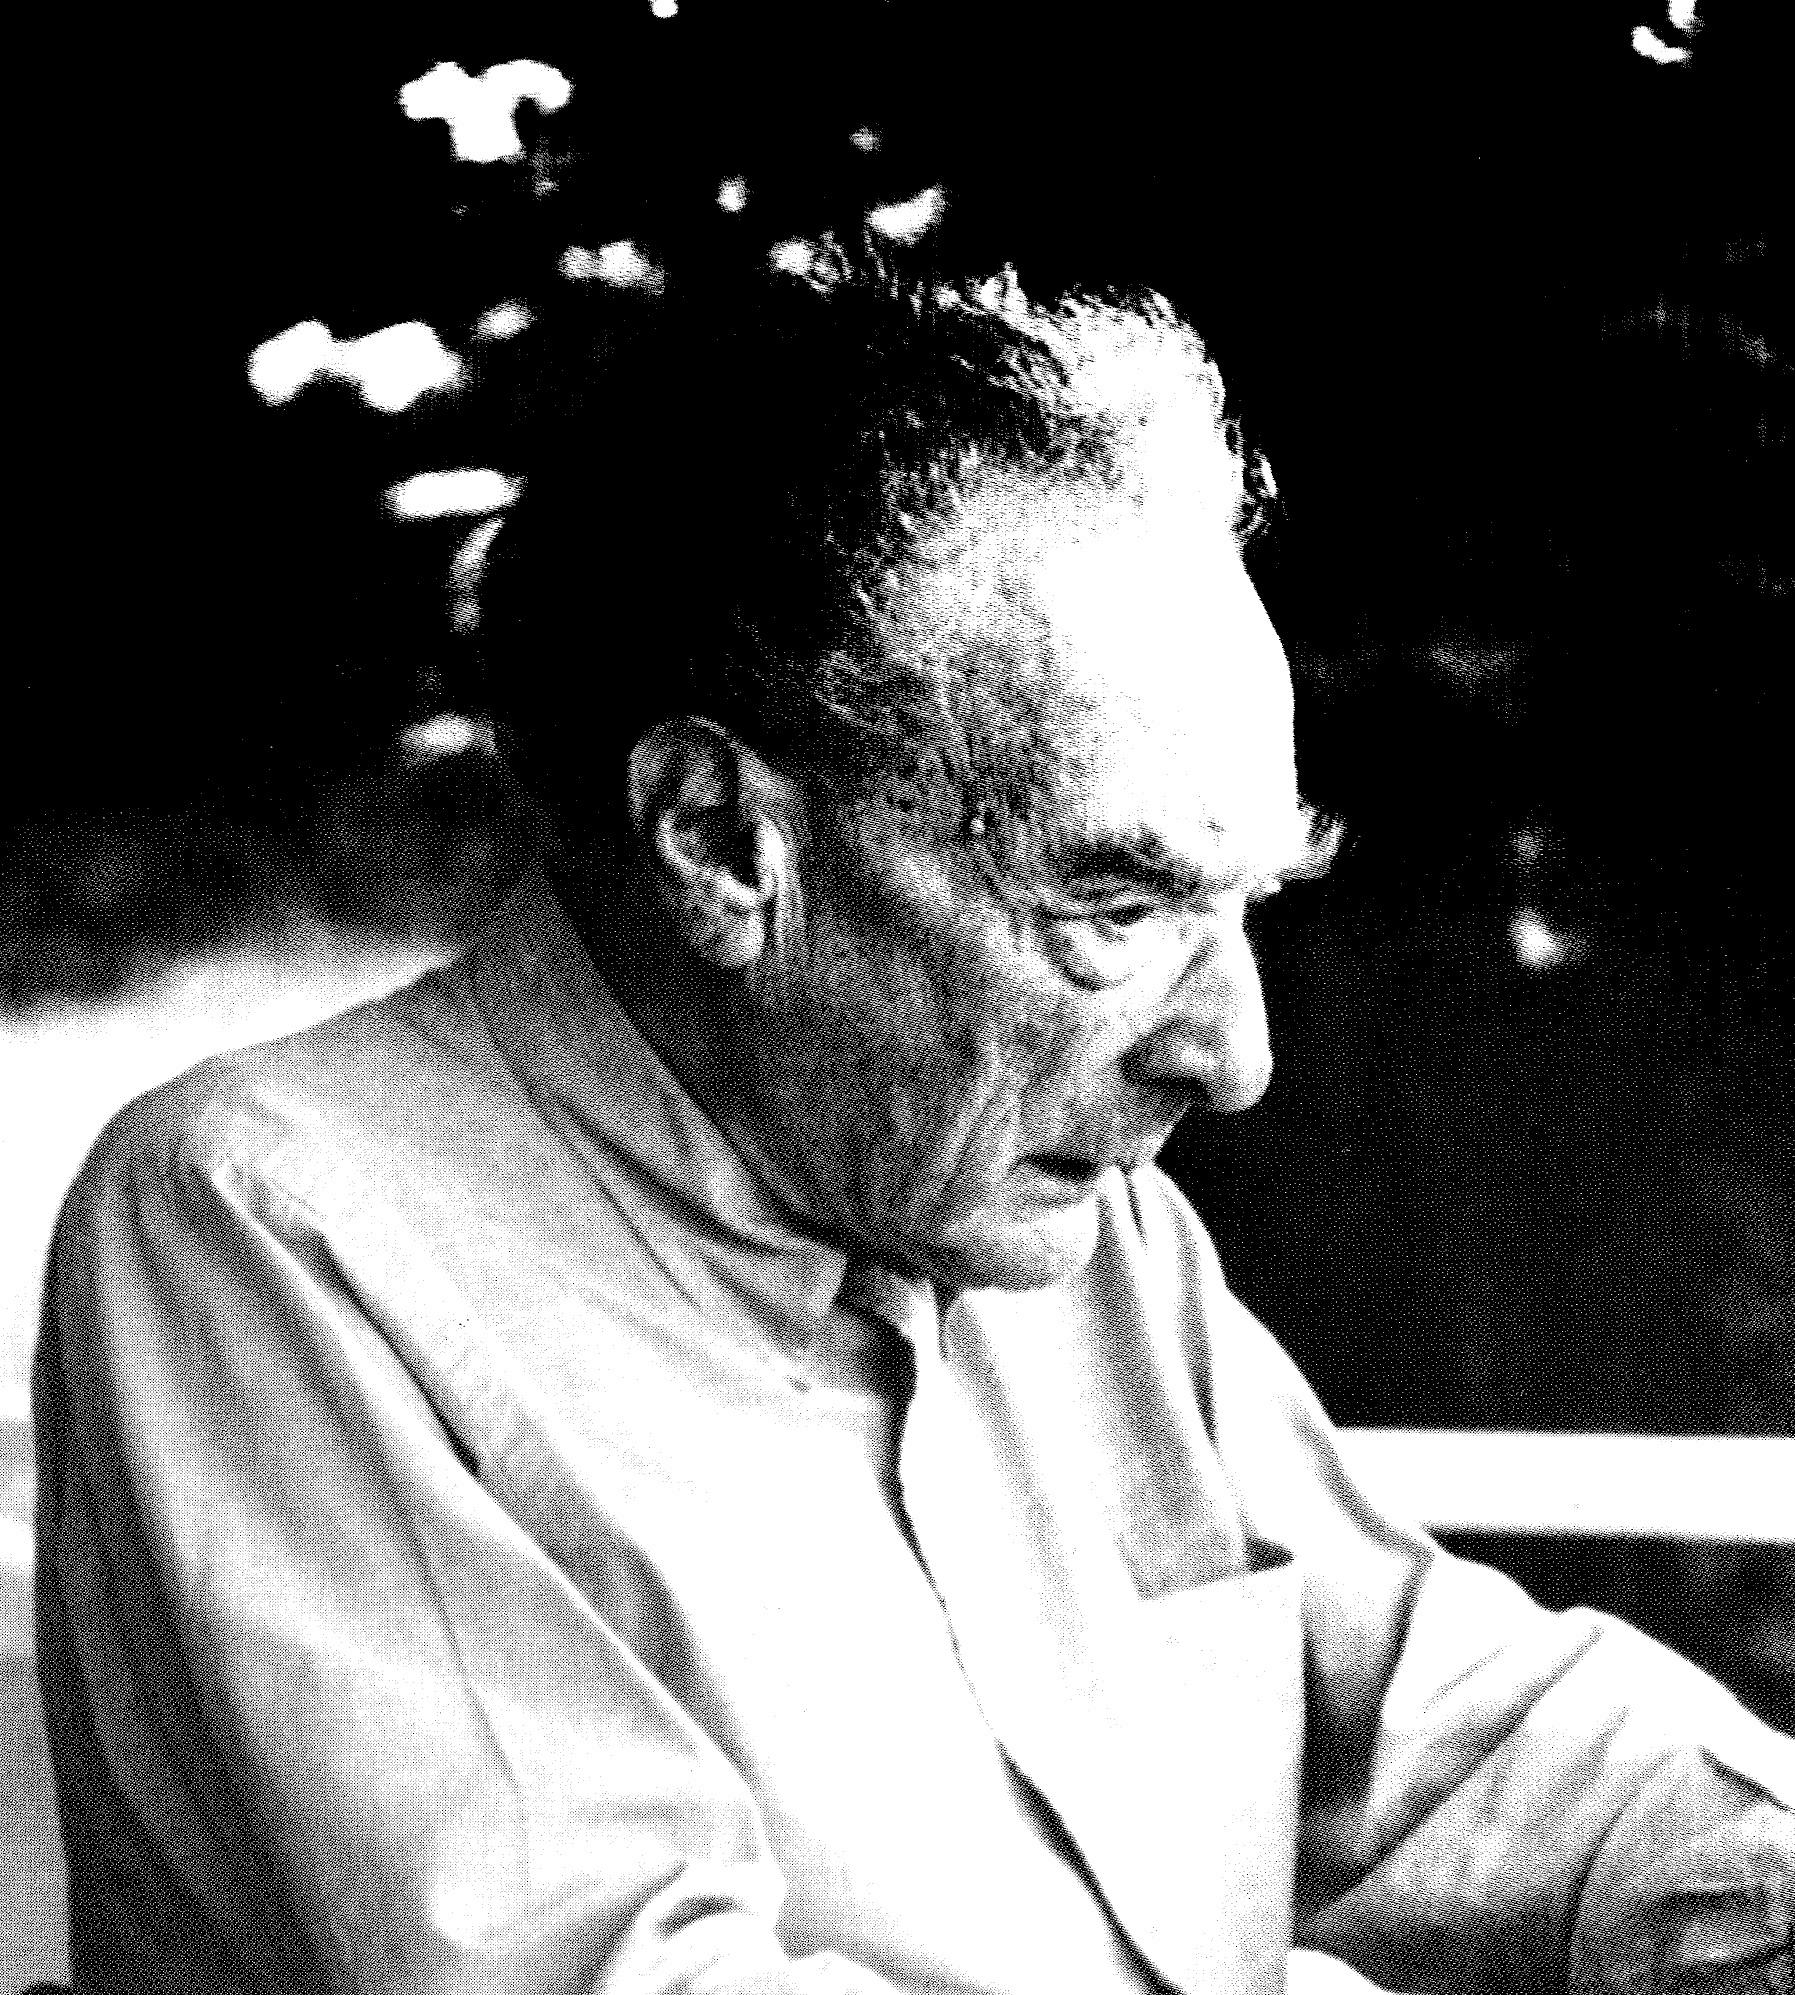
\includegraphics[width=.9\textwidth]{figures/Jakobson-lsa.jpg}
  \caption{Roman Jakobson in later years}
  \label{fig:ch.jakobson_jakobson_lsa}
\end{wrapfigure}
Clearly, much of the conceptual capital of generative phonology was
inherited from {\Jakobson}'s work (as will be discussed further in
chapter~\ref{ch.genphon}). The basic system of \isi{distinctive features},
despite the modifications it has undergone in subsequent work, has its
roots firmly in {\Jakobson}'s theory. Similarly, the basic research goals
of phonological investigation, including the formulation of
explanatory general laws, and the integration of accounts of
\isi{historical change}, language acquisition, and language pathology into a
theory of synchronic systems, were most forcefully expressed in his
work. Nonetheless, not all of the foundations of his views (when these
are made explicit) would find general acceptance among later
phonologists; and it is important to examine particular points derived
from those views to see how comfortably they can be integrated into
our present framework of assumptions.

%%% Local Variables: 
%%% mode: latex
%%% TeX-master: "/Users/sra/Dropbox/Docs/Books/P20C_2/LSP/main.tex"
%%% End: 
